\documentclass[twocolumn,10pt]{article}
\usepackage{luad_biorxiv}
\graphicspath{{figs/}}

\begin{document}

\twocolumn[%
  \frontblock{%
    Paired single-nucleus and spatial transcriptomics of the lung adenocarcinoma
    invasion sequence reveal niche domains and candidate reversal compounds}%
  {Zhiyang Li\textsuperscript{1,$\ast$}\quad Jiaxuan Yang\textsuperscript{2}}%
  {\textsuperscript{1}Guangdong Medical University, Zhanjiang, Guangdong, China\\[0.2em]
   \textsuperscript{2}Monash University Malaysia, Bandar Sunway, Selangor, Malaysia}%
  {\textsuperscript{$\ast$}Correspondence: Zhiyang Li, \texttt{eto-1024@gdmu.edu.cn}}%
  \frontabstract{Lung adenocarcinoma (LUAD) develops through a defined morphological sequence from atypical
adenomatous hyperplasia (AAH) to invasive adenocarcinoma, but the transcriptional programmes
accompanying this transition have mostly been characterised in bulk tissue or in tumour
tissue alone. We profiled paired samples spanning the full sequence by single-nucleus RNA
sequencing (413,697 nuclei, 23 patients) and spatial transcriptomics (56 Visium sections, 25
patients), asking how the transcriptional state of the tissue changes as invasion proceeds
and whether that state can be reversed \emph{in silico} by known perturbations.

The atlas resolves into 39 second-level subtypes and the tissue into seven recurring
niche-domain archetypes ($K^{*}=7$), six of which are ordinary lung structures and only one
of which is restricted to invasive disease. A confound then shaped the remaining analyses:
domain identity, marker stability and the apparent stage-dependence of the spatial programmes
all scale with sequencing depth, and depth is in these sections a proxy for tissue density
rather than a purely technical artefact ($\rho=-0.89$ between a domain's depth and the
fraction of its markers surviving depth matching). Several apparently positive results
disappeared once depth was matched. The invasive domain's ECM/interstitial identity survives
that check: within patients the fibroblast ECM programme is higher in invasive disease in 20
of 22 paired cases ($P=0.0033$ against random gene sets), and the result is unchanged when
the genes added by hand are removed and under every leave-one-out variant.

Querying a patient-paired disease axis against the LINCS compound library with three scoring
schemes returned 34 compounds in common, dominated by PI3K/mTOR inhibitors, with a
split-half reproducibility of $\rho=0.962$ against a permutation null of $\pm0.045$ and an
agreement of $\rho=0.735$ between a single-cell-derived and a spatially derived axis. A
positive control, the recovery of known regulators of an official benchmark (TBXT ranked 1st
of 8,450), establishes that the pipeline recovers true positives, so the negative results
reported here are properties of the data rather than of the method. Those negatives are
stated explicitly: single-cell copy-number inference produced no usable
malignant/non-malignant separator, the cohort-level spatial copy-number difference did not
survive depth matching, a developmental trajectory ran opposite to that of the source study,
gene-level prediction returned no signal on the pooled axis and only one perturbation
survives compartment-wise gating, and a ligand-level analysis produced no usable pair.
}%
]%

\section{Introduction}

Lung adenocarcinoma (LUAD) develops through a stereotypic morphological sequence that
begins with atypical adenomatous hyperplasia (AAH) and proceeds through adenocarcinoma
\emph{in situ} (AIS) and minimally invasive adenocarcinoma (MIA) to invasive
adenocarcinoma (IAC). Each stage is histologically defined, and the transition from
precursor lesion to invasive carcinoma is the point at which clinical management changes.
The sequence therefore provides a well-defined system in which to ask what transcriptional
changes accompany invasion and in what order they arise.

Most transcriptomic descriptions of this sequence derive either from bulk tissue
\citep{tcga2014luad} or from single-cell profiling restricted to the invasive tumour and
adjacent normal lung, and both designs conflate the intermediate states that define the
sequence. Single-cell atlases spanning the full spectrum are available \citep{han2024}, but
these rarely carry a spatially resolved counterpart, so the tissue architecture surrounding
a given transcriptional state, such as the niche composition around an alveolar type II
cell, remains unobserved.

Two obstacles are specific to this disease. Tumour cells are difficult to identify without
copy-number information, because the reference panels used for spatial deconvolution
contain no malignant cell type; malignant epithelium is assigned to the most similar normal
epithelial class, leaving any composition-based description of a niche structurally blind
to the tumour. In addition, invasive regions of a section are both more cellular and more
transcriptionally active than precursor regions, so comparisons between the two are also
comparisons of RNA content.

We assembled paired single-nucleus RNA sequencing and Visium spatial transcriptomics from
23 patients spanning all five stages. The single-cell data define cell states and a
patient-internal disease axis. The spatial data define tissue niches
\citep{singhal2024banksy,cable2022rctd} and provide the context in which the copy-number
signal is placed \citep{cabrejas2026fastcnv}. The same disease axis is then used as a query
against two perturbation libraries \citep{subramanian2017}, to ask whether any known
compound or gene perturbation reverses it.

A methodological result obtained early shaped the remainder of the study. Sequencing depth
and tissue density are not separable in this cohort, and their coupling is strong enough to
generate stage-dependent patterns where none exist. Controlling for it, and reporting what
survives when that control is incomplete, became the organising constraint of the work. We
therefore present positive and negative results together and record the analytical
difficulties encountered, several of which required the withdrawal of an apparently sound
result.

\section{Results}

\subsection{A single-nucleus atlas of the LUAD invasion sequence}

Paired single-nucleus RNA sequencing and Visium spatial transcriptomics were obtained from
23 patients spanning the five stages of the sequence, with the spatial arm covering 56
sections from 25 patients and sharing 23 patients with the single-cell arm
(Fig.~\ref{fig:1}a). Quality control retained 399,579 nuclei. The atlas resolves into six
lineages (epithelial, fibroblast, endothelial, myeloid, T/NK, B/plasma;
Fig.~\ref{fig:1}a) and, on per-lineage sub-clustering, into 39 second-level (L2) subtypes
(Supplementary Table~S1; Fig.~\ref{fig:1}f).

Two properties of the reference annotation affected the analyses that follow and are
recorded here.

\emph{Endothelial and myeloid panels were rebuilt.} The published marker table supplies six
canonical genes per endothelial subtype, which is insufficient to discriminate between
closely related endothelial states. Under that panel the \emph{Artery} subtype was assigned
to 16 clusters across the cohort; under an expanded panel of up to 20 genes per subtype
across nine endothelial types it was assigned to four, with the remainder reassigned to
\emph{Lymphatic}, \emph{Vein} and \emph{Capillary}. The endothelial and myeloid panels were
therefore rebuilt before any downstream analysis. Analyses that depend on endothelial
subtype proportions inherit the corrected panels.

\emph{The L2 nomenclature is not a set of unique identifiers.} The 39 names map onto 67
distinct lineage--subtype combinations. The clearest case is \emph{Basophil/Mast 1}, which
the reference assigns predominantly to epithelial cells (6,360 cells) and only marginally
to myeloid cells (8 cells), so the name misrepresents the content. Subtype composition is
accordingly reported at the lineage level (Fig.~\ref{fig:1}e).

A second difficulty concerns the coverage rather than the nomenclature of the reference. The
39-subtype reference contains no exhaustion programme, and exhausted T cells were
consequently absorbed into the nearest available label. One cluster carries LAG3, TIGIT,
HAVCR2, ENTPD1, GZMB and PRF1 while lacking CCR7, SELL, TCF7 and LEF1, an exhausted rather
than a naive phenotype, yet the reference assigns it to \emph{CD8+ Naive T}. Deconvolution
cannot recover a state absent from the reference, so the T-cell composition reported here is
a composition in the reference's vocabulary. Functional exhaustion was therefore measured
independently, by projecting an exhaustion signature
\citep{thommen2018,wherry2015exhaustion} onto the spots.

One AAH sample (P24) carried a plasma-cell programme confined to a single patient and not
tracking disease stage. A patient-level rank of B/plasma content, comparison against a
matched negative-control gene set, and an independent readout from a separate region of the
same block each identified it as ambient RNA rather than a tumour-associated infiltrate. The
sample was retained with an annotation, and all conclusions that depend on B/plasma content
are reported both with and without it. The source study does not describe ambient-RNA
correction, and P24 is one of its representative samples.

\begin{figure*}[!ht]\centering
  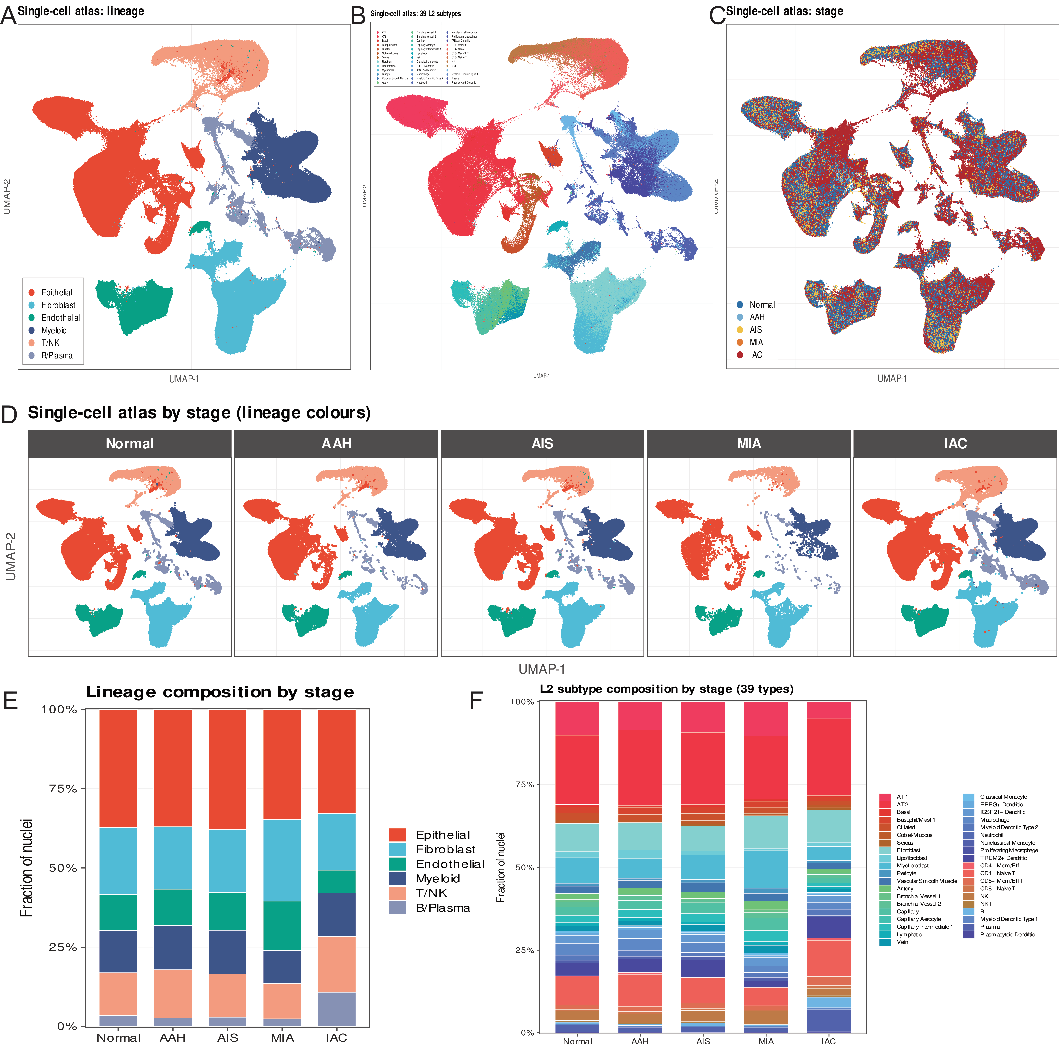
\includegraphics[width=\textwidth]{Fig1}
  \caption{\textbf{A single-nucleus atlas of the LUAD invasion sequence.}
(\textbf{a}) UMAP of 399,579 nuclei coloured by lineage.
(\textbf{b}) Lineage composition across the cohort.
(\textbf{c}) The same embedding coloured by disease stage.
(\textbf{d}) The embedding split by stage, retaining lineage colours.
(\textbf{e}) Lineage composition per stage.
(\textbf{f}) Composition of the 39 second-level subtypes per stage.
Endothelial and myeloid marker panels were rebuilt before composition analysis (Methods).
The 39 subtype names are not unique lineage--subtype identifiers (67 combinations);
compositions are reported at the lineage level in (\textbf{e}).}\label{fig:1}
\end{figure*}


\subsection{Spatial deconvolution resolves seven recurring niche domains}

BANKSY applied per section yielded 434 spatial domains, which collapsed to seven archetypes
($K^{*}=7$; cross-seed stability 0.945) across the 56 sections (Fig.~\ref{fig:2}d).
Stability falls to 0.814 at $K=8$, so the domains cannot be subdivided further without
becoming seed-dependent. We therefore treat $K^{*}=7$ as the resolution limit of this
cohort. A purely descriptive optimum exists at $K=6$ (stability 0.966) and was not adopted.

Identities were assigned from each archetype's RCTD composition (Fig.~\ref{fig:2}a,c) and
its marker genes (Fig.~\ref{fig:2}g). Six of the seven are ordinary lung structures: airway
epithelium (D1), peribronchovascular interstitium carrying an inflammatory CAF programme
(D2) \citep{ohllund2017,elyada2019}, alveolar wall (D4), AT2 epithelium (D5), vascular and
airway smooth muscle (D6), and lymphocyte aggregates (D7). Only D3 is restricted to
invasive disease. On the stage axis (Fig.~\ref{fig:2}d), D3 accounts for 17\% of spots in
IAC and \textbf{0\% in every precursor stage}, whereas D7 is present in all five stages.
The presence of lymphoid aggregates before invasion argues against the assumption that
immune aggregation accompanies malignancy.

Two caveats attach to the domain labels. The published marker table for these domains is
itself depth-confounded (see below), and the identity of D3 was revised twice during the
study, from an immune-infiltrate reading to a hypoxic/invasive reading and then to its
current ECM/interstitial reading; the earlier names should not be used. The domain
definition is also method-sensitive: BANKSY, RCTD composition and marker-based clustering
return 7, 6 and 5 domains respectively, with an adjusted Rand index of only 0.225--0.247
against an RCTD-aligned partition. Domain boundaries are therefore quantitative but not
unique. The composition underlying each label is given in Table~\ref{tab:domains}.

\begin{figure*}[!ht]\centering
  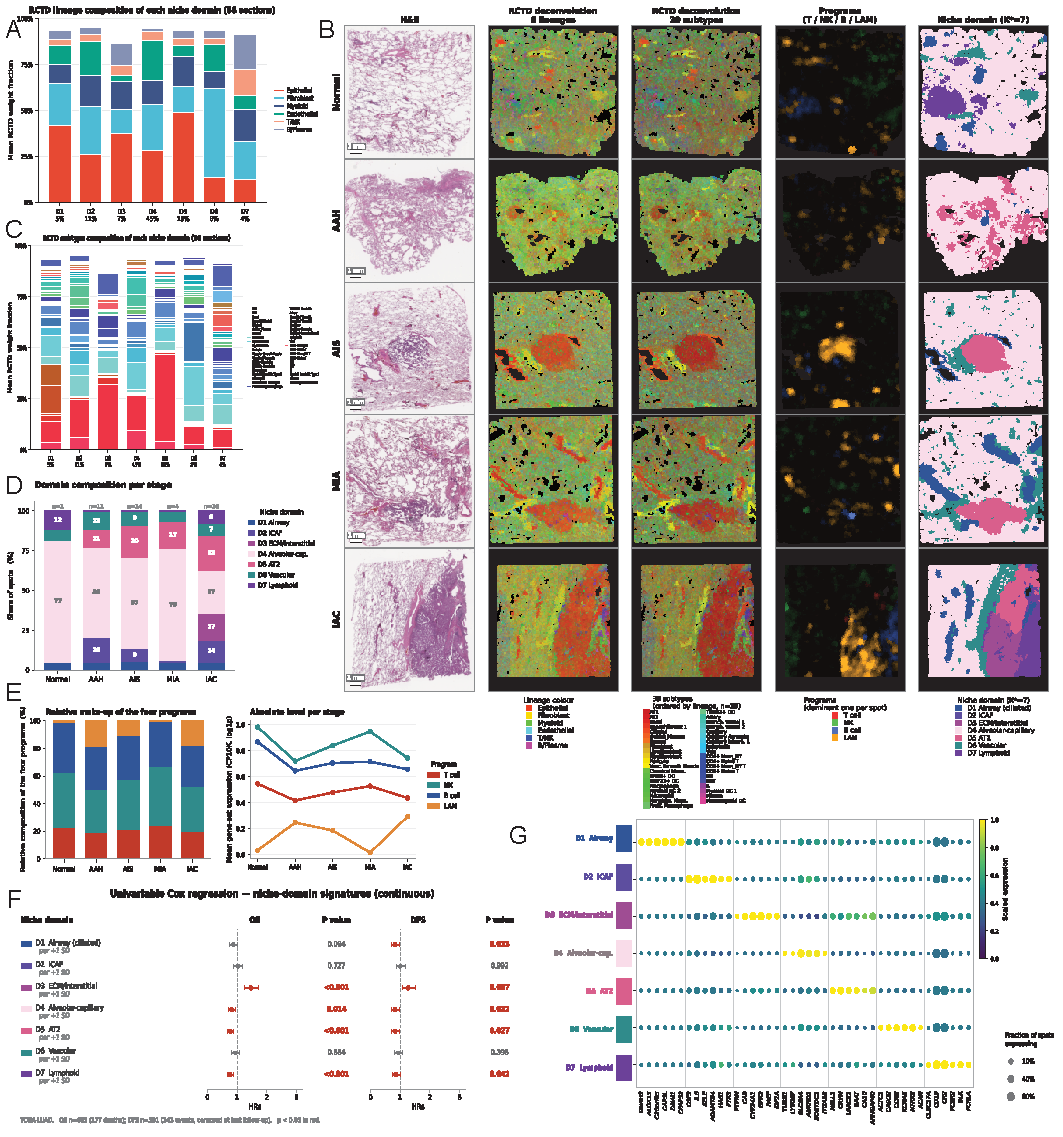
\includegraphics[width=\textwidth]{Fig2}
  \caption{\textbf{Spatial deconvolution resolves seven niche-domain archetypes.}
(\textbf{a}) RCTD lineage composition of each domain archetype (56 sections).
(\textbf{b}) Spatial matrix: one representative section per stage (rows) against
H\&E, RCTD at the 6-lineage and 39-subtype level, the four spatial programmes
(dominant programme per spot) and the niche-domain archetype (columns). Scale bars are
calibrated per section from the nominal 100-$\mu$m spot spacing.
(\textbf{c}) RCTD subtype composition of each domain archetype.
(\textbf{d}) Domain composition per stage; D3 is confined to invasive disease
(17\% of spots, 0\% in all precursor stages) whereas the lymphoid domain D7 occurs in all
five stages.
(\textbf{e}) Relative make-up and absolute level of the four spatial programmes per stage.
\textbf{This panel is a negative control}: before depth matching the programme scores
essentially mirror sequencing depth, and after matching into depth deciles the stage
ordering is identical across all ten deciles but does not follow disease progression. The
fourth programme is the lipid-associated macrophage (LAM) signature \citep{cheng2021trem2lam},
which we report alongside three exhaustion axes; it is not an exhaustion signature in the
T-cell sense.
(\textbf{f}) Univariable Cox regression of each domain's marker signature on overall and
disease-free survival (TCGA-LUAD); p\,$<$\,0.05 in red. The D3 row uses the unadjusted
signature (see main text).
(\textbf{g}) Marker-gene dot plot for the seven domains.}\label{fig:2}
\end{figure*}


\begin{table*}[!ht]
\centering
\begin{tabularx}{\textwidth}{@{}>{\bfseries}l >{\raggedright\arraybackslash}p{86pt} >{\raggedright\arraybackslash}p{152pt} >{\raggedleft\arraybackslash}p{50pt} >{\itshape\raggedright\arraybackslash}X@{}}
\toprule
\tabheadfont Domain & \tabheadfont Label & \tabheadfont Basis (RCTD enrichment or depth-balanced markers) & \tabheadfont Share & \tabheadfont Note \\
\midrule
D1 & Airway epithelium & Ciliated $\times$6.3; Goblet $\times$5.6 & 5\% & \\
D2 & iCAF stroma & IL6, CXCL8, CCL2, LIF, HAS1, HAS2 & 11\% & peribronchovascular \\
D3 & ECM / interstitial & COL1A1, COL3A1, FN1, CTHRC1 & 17\% (IAC) & no precursor stage; two label revisions \\
D4 & Alveolar wall & Capillary $\times$2.5; AT1 $\times$1.9 & 45\% & 77\% of the Normal section \\
D5 & AT2 epithelium & AT2 weight 0.480 ($\times$2.0) & 19\% & highest copy-number score \\
D6 & Vascular / airway wall & VSMC $\times$5.1; Artery $\times$2.3 & 8\% & \\
D7 & Lymphoid aggregate & B $\times$9.1; NKT $\times$4.7 & 4\% & present in all five stages \\
\bottomrule
\end{tabularx}
\caption{\textbf{Identity of the seven niche-domain archetypes.} Enrichment is the RCTD
composition of a domain relative to the rest of the cohort, as a fold change; the share is
the fraction of all spots assigned to that domain. The D3 label was revised twice during
the study (see main text) and the earlier names should not be used. No label here implies a
malignancy call.}
\label{tab:domains}
\end{table*}


\subsection{Sequencing depth is a proxy for tissue density}

The seven domains differ in sequencing depth by a factor of 1.00 to 7.95. Depth matching
removes a large and predictable fraction of each domain's marker genes: across the seven
domains, the fraction of a domain's top-150 up-genes surviving per-slide depth matching
falls monotonically with depth (Spearman $\rho=-0.89$; Fig.~\ref{fig:3}f), with two
independent estimators (decile matching and per-gene regression on $\log_{10}$(nUMI))
agreeing almost gene-for-gene. D3 is the sole outlier; it is both the deepest domain and the
only one restricted to invasive disease, and 16 of its 150 markers survive matching.

This resembles a standard technical confound, and treating it as one would be an error. The
same quantity is independently visible in the images: the PLIP-derived neoplastic score
correlates with the fraction of a spot occupied by tissue at $\rho=0.754$ across four
sections of one patient. Deep spots are therefore deep because they are dense, and dense
because they contain tumour. Removing depth as a covariate removes part of the biological
signal; the operation is closer to over-adjustment than to deconfounding, and neither the
unadjusted nor the adjusted estimate is correct on its own.

This coupling is the binding constraint of the study and recurs in four places. In the
spatial copy-number arm it determines which comparisons survive. In the prognosis arm it is
the reason one domain's apparent prognostic effect shrinks when its signature is replaced by
a depth-balanced version. In the developmental analysis it accounts for a trajectory running
opposite to that of the source study. It also prevents interpretation of the
stage-dependence of the four spatial programmes. Before matching, their scores are almost a
mirror of depth (per-spot $r=-0.30$ to $-0.69$ for the T-cell programme; sections differ
2.4-fold in median depth). After matching into depth deciles the stage ordering is identical
across all ten deciles but does not follow disease progression: AAH and AIS are both
precursor stages yet occupy opposite ends of the ordering. That comparison is consequently
reported as a negative control (Fig.~\ref{fig:2}e).

Because the revised identity of D3 is an ECM/interstitial programme, that programme was
tested directly rather than accepted from the domain analysis. Within each patient,
fibroblasts were scored against the cohort fibroblast mean and standard deviation per gene,
and the mean of a 22-gene ECM set was compared between invasive and precursor fibroblasts.
The programme is higher in invasive disease in \textbf{20 of the 22 patients with both
stages} (median within-patient difference $+0.402$; 300 random gene sets of matched size
drawn from expressed genes give $P=0.0033$ on both the count and the median). Eight of the
22 genes were added by us rather than drawn from the depth-balanced D3 ranking; restricting
the panel to the 14 data-derived genes gives 20 of 22 ($+0.347$, $P=0.0033$), restricting it
to the eight hand-added genes also gives 20 of 22 ($+0.450$, $P=0.0033$), and removing any
single gene leaves the count at 20 of 22 in all 22 leave-one-out variants. The ECM programme
is therefore not an artefact of gene selection, although the result describes a tissue-level
programme in fibroblasts and does not identify which ECM component is responsible.

\subsection{Copy-number inference: three failures and one surviving signal}

Malignant-cell identification is where the analytical failures of this study concentrate,
and they are reported in full because they constrain the interpretation of the spatial
results.

\paragraph{Single-cell inference.} Across six tool families, comprising CopyKAT
\citep{gao2021copykat} in default and floored configurations, two anchor-based arms, inferCNV
v1 and v2 \citep{patel2014infercnv}, and a supervised expression-based classifier
\citep{scmalignantfinder2025}, no configuration produced a usable malignant/non-malignant
separator, and each failure was traced to a specific cause. The clearest was an instability
check: the same set of 3,890 normal cells, used as the reference in three separate runs,
produced aneuploid calls of 0\%, 13.6\% and 49.8\%. The most misleading was an AUROC of
exactly 0.5000 from inferCNV v1, where all 19,748 cells carried a single identical score
value because the per-cell statistic reduced to the constant reference baseline; the ROC was
a degeneracy rather than evidence of an absent difference. A second version produced AUROC
0.652 but failed its own control, the normal cells scoring 0.0826 against a threshold of
0.05.

\paragraph{Cohort-level spatial copy number.} All 25 cases ran successfully at the Visium
level. The cohort-level claim that invasive sections carry more copy-number signal shrank by
71\% after depth balancing, and the matched comparison was not significant ($p=0.092$,
confidence interval including zero). A random subsample reproduced the pre-matching result
index by index, confirming that the original effect was driven by sequencing depth rather
than by sample size. No cohort-level copy-number difference is therefore reported.

\paragraph{One comparison survives by design.} Comparing each domain against the remaining
spots of the same section removes depth by construction, since every spot in the comparison
shares one cDNA library (Fig.~\ref{fig:3}c). Under this design the copy-number score is
elevated in D5 (AT2; median $\Delta=+0.044$, positive in 40 of 46 sections, $p<0.001$) and
in D3 (12 of 12 sections, $p=0.0005$); D4, D6 and D2 are significantly lower, and D1 and D7
show no effect. Restricted to precursor sections, D5 remains positive in 17 of 20, so the
signal is present before invasion. This is consistent with AT2 as the cell of origin in this
disease and with an independent supervised classifier whose signal was likewise confined to
AT2.

The score is a continuous quantity and not a malignancy call; no malignant label is assigned
to any spot or domain. Within D5, splitting spots into high and low copy-number groups
produces spatially coherent patches, but the split is not separable from RNA content: the
correlation between score and total UMI within D5 is $r=0.740$, and splitting by spot counts
alone reproduces roughly 75\% of the difference in AT2 content between the two groups. A
``D5-high'' subdomain therefore cannot be described as a tumour subdomain.

\subsection{Prognostic association of the niche domains}

The domain marker signatures were tested for prognostic information in an independent cohort
(TCGA-LUAD; 483 patients, 177 deaths; 381 patients and 143 events for disease-free survival).
Using each domain's top-30 markers standardised across samples, the associations are
consistent between a continuous parameterisation and a median split (Fig.~\ref{fig:2}f) and
between overall and disease-free survival. A high D7 (lymphoid) signature is associated with
better outcome (continuous HR 0.77, $p<0.001$; median split HR 0.60) and a high D3 signature
with worse (HR 1.46, $p<0.001$; HR 2.03); D4 and D5 are protective on overall survival.

The D3 result requires qualification. Its signature is drawn from the raw marker table,
which the depth analysis shows to be dominated by depth for this domain. Replacing it with
the depth-balanced signature reduces the adjusted hazard ratio from 2.30 to 1.30
($p=0.09$), and the connectivity-map signal for the same signature falls within the random
range. The direction and its robustness are therefore reported, but not the point estimate,
and D3 is not treated as an established prognostic feature.

\subsection{\emph{In-silico} reversal of the disease state}

To ask whether the disease state can be reversed, a query signature was derived from the
single-cell data and used against two perturbation libraries.

\paragraph{Query construction.} For each patient the difference in mean expression between
invasive and precursor cells was computed and the median taken across patients, giving a
16,104-gene axis. This axis was filtered against an independent survival signal (per-gene
adjusted Cox models in TCGA-LUAD), retaining a gene only where the direction of disease
change agreed with the direction of prognostic effect, so that a gene rising in disease is
retained only if higher expression also predicts worse outcome, and conversely
(Fig.~\ref{fig:3}a). The filter removes 9,270 of 18,069 genes (51\% of the full set; 44\% of
the 15,792 genes with survival data), of which 6,993 change in disease but are protective
and 2,277 lack survival annotation. It is applied because a reversal query that ignores it
would target protective programmes as readily as harmful ones.

\paragraph{Scoring schemes.} The signature was scored against the LINCS library using the
CMap weighted-KS statistic ($\tau$) and two correlation-based scores. The library was rebuilt
and held locally rather than queried through the CLUE scoring service, which was retired on
2026-01-31 (Methods), so the version queried is fixed and re-runnable and every scoring path
is cross-validated against the official implementation. The two correlation scores are
nearly redundant (Spearman $\rho=0.950$; 433 of 1,826 compounds shared in their top 500),
whereas the CMap statistic shares only about a third of its ranking with them
($\rho=0.36$--$0.38$; 18--19 of 50 in the top 50) (Fig.~\ref{fig:3}h). This reflects the
statistics rather than the implementation: CMap-type scores use only the membership of the
query's gene sets and discard the perturbation values, and are therefore systematically
different from value-based correlations. Requiring a compound to rank in the top 100 under
all three schemes is consequently a stricter filter than it appears, and yields
\textbf{34 compounds} (chance expectation 5.5), of which 16 (47\%) target PI3K/mTOR, with
smaller groups against HSP90, the proteasome and cell-cycle kinases (Fig.~\ref{fig:3}d; Table~\ref{tab:compounds}).

\begin{table*}[!ht]
\centering
\begin{tabular*}{\textwidth}{@{\extracolsep{\fill}}lrS[table-format=-1.3]S[table-format=-1.3]S[table-format=-1.3]rr@{}}
\toprule
\multicolumn{1}{@{}l}{\tabheadfont Compound} & \multicolumn{1}{l}{\tabheadfont Mechanism} & \multicolumn{1}{c}{\tabheadfont CMap $\tau$} & \multicolumn{1}{c}{\tabheadfont Cor-Sp $\rho$} & \multicolumn{1}{c}{\tabheadfont Cor-Pr $\rho$} & \multicolumn{1}{c}{\tabheadfont Rank CMap} & \multicolumn{1}{c@{}}{\tabheadfont Rank Cor-Sp} \\
\midrule
AZD-2014 & PI3K / mTOR & -0.355 & -0.186 & -0.112 & 1 & 15 \\
lacidipine & PI3K / mTOR & -0.330 & -0.188 & -0.113 & 2 & 14 \\
AZD-8055 & PI3K / mTOR & -0.329 & -0.176 & -0.111 & 3 & 23 \\
PKI-179 & PI3K / mTOR & -0.322 & -0.223 & -0.152 & 5 & 2 \\
GDC-0941 & PI3K / mTOR & -0.311 & -0.111 & -0.071 & 7 & 61 \\
MLN-0128 & PI3K / mTOR & -0.311 & -0.205 & -0.128 & 8 & 8 \\
NVP-AUY922 & HSP90 & -0.304 & -0.135 & -0.091 & 9 & 46 \\
GDC-0980 & PI3K / mTOR & -0.302 & -0.215 & -0.137 & 10 & 5 \\
BIIB-021 & JAK2 & -0.294 & -0.170 & -0.118 & 13 & 28 \\
taselisib & PI3K / mTOR & -0.291 & -0.146 & -0.116 & 14 & 41 \\
okadaic acid & phosphatase & -0.286 & -0.179 & -0.142 & 18 & 20 \\
XL-888 & cell-cycle kinase & -0.280 & -0.223 & -0.134 & 20 & 3 \\
JW-7-24-1 & mTOR & -0.279 & -0.094 & -0.065 & 22 & 87 \\
torin-2 & PI3K / mTOR & -0.277 & -0.237 & -0.153 & 23 & 1 \\
midostaurin & kinase & -0.276 & -0.109 & -0.059 & 24 & 62 \\
NVP-BEZ235 & PI3K / mTOR & -0.274 & -0.199 & -0.124 & 26 & 10 \\
bortezomib & proteasome & -0.271 & -0.180 & -0.106 & 29 & 19 \\
pentobarbital & GABA-A & -0.266 & -0.163 & -0.093 & 30 & 33 \\
PI-103 & PI3K / mTOR & -0.264 & -0.155 & -0.093 & 31 & 36 \\
TAK-285 & HER2 / EGFR & -0.261 & -0.117 & -0.081 & 32 & 57 \\
voxtalisib & PI3K / mTOR & -0.257 & -0.093 & -0.063 & 35 & 91 \\
torin-1 & PI3K / mTOR & -0.250 & -0.149 & -0.094 & 40 & 39 \\
PF-03814735 & Aurora kinase & -0.242 & -0.119 & -0.067 & 42 & 55 \\
AT-13387 & HSP90 & -0.237 & -0.154 & -0.089 & 48 & 37 \\
OSI-027 & mTOR & -0.236 & -0.093 & -0.062 & 51 & 89 \\
WYE-125132 & mTOR & -0.217 & -0.172 & -0.107 & 69 & 25 \\
MG-132 & proteasome & -0.214 & -0.184 & -0.109 & 72 & 16 \\
NVP-TAE226 & FAK & -0.213 & -0.164 & -0.101 & 73 & 32 \\
GSK-2110183 & PI3K / mTOR & -0.209 & -0.101 & -0.081 & 77 & 79 \\
dinaciclib & CDK & -0.208 & -0.177 & -0.102 & 82 & 22 \\
GSK-2126458 & PI3K / mTOR & -0.208 & -0.218 & -0.139 & 83 & 4 \\
YM-155 & survivin & -0.205 & -0.140 & -0.075 & 87 & 42 \\
tanespimycin & HSP90 & -0.205 & -0.183 & -0.118 & 88 & 17 \\
SB-939 & cell-cycle kinase & -0.199 & -0.102 & -0.059 & 94 & 77 \\
\bottomrule
\end{tabular*}
\caption{\textbf{The 34 compounds common to all three scoring schemes.} Compounds rank in
the top 100 under each of the CMap weighted-KS statistic ($\tau$) and the two correlation
scores, applied to the prognosis-filtered patient-internal disease axis against the LINCS
library (1{,}826 compounds). Rows are ordered by CMap rank. Values are medians across the
cell lines in which a compound was profiled; more negative indicates stronger reversal. The
chance expectation for a compound to appear in all three top-100 lists is 5.5. Mechanisms
are annotated from library metadata, curated for incompletely annotated compounds; the
assignment plays no part in selection.}
\label{tab:compounds}
\end{table*}


\paragraph{Reproducibility and modality independence.} Splitting patients at random into
halves, deriving the axis independently in each half and scoring both against LINCS
reproduces the ranking with a median Spearman $\rho$ of 0.962 across four splits, against a
permutation null of $\pm0.045$ (Fig.~\ref{fig:3}e, left); the top-500 lists share 438
compounds on average against a chance expectation of 137. One split is weaker ($\rho=0.752$)
and all four are reported. A second query axis was derived from the spatial data, after
depth balancing, by comparing invasive and precursor spots within nUMI deciles, and scored
against the same library with the same statistic. The two axes agree at Spearman
$\rho=0.735$ (top-100 overlap 52, chance expectation 5.5) (Fig.~\ref{fig:3}e, right). Since
the two axes derive from different platforms and different pairing strategies, this is a
stronger reproducibility check than repeating the scoring scheme within one modality.

\paragraph{Positive control.} Before the candidate list was examined, the pipeline was
verified against an official benchmark with a known answer, the epiblast-to-nascent-mesoderm
transition, using the authors' own implementation, manifold and standard deviations
\citep{pan2026scmg}. The known regulators are recovered at the top of the ranking: TBXT 1st
of 8,450, MSGN1 2nd, MIXL1 3rd, POU5F1 7th, SNAI1 9th, EOMES 11th, NANOG 12th and EVX1 15th
(Fig.~\ref{fig:3}b). This establishes that an empty result from the pipeline indicates the
query or the data rather than a broken method. Numerical identity with the official
implementations was confirmed separately: the weighted-KS implementation reproduces the
reference to a maximum absolute difference of $6.6\times10^{-14}$ with 2000 of 2000 signs
agreeing, and the vectorised causal score reproduces the authors' Python at Spearman
1.00000000. Table~\ref{tab:validation} collects these and the other numerical agreements
reported below.

\paragraph{The reversal acts on specific domains.} Using each domain's own depth-balanced
signature as a query, 26 of the 34 candidates fall in the top 100 for D3 and 21 for D5,
against a chance expectation of 1.9; the remaining five domains are at or near chance
(Fig.~\ref{fig:3}g). The compounds therefore act on the ECM/interstitial and AT2 domains
rather than on the tissue as a whole.

\begin{figure*}[!ht]\centering
  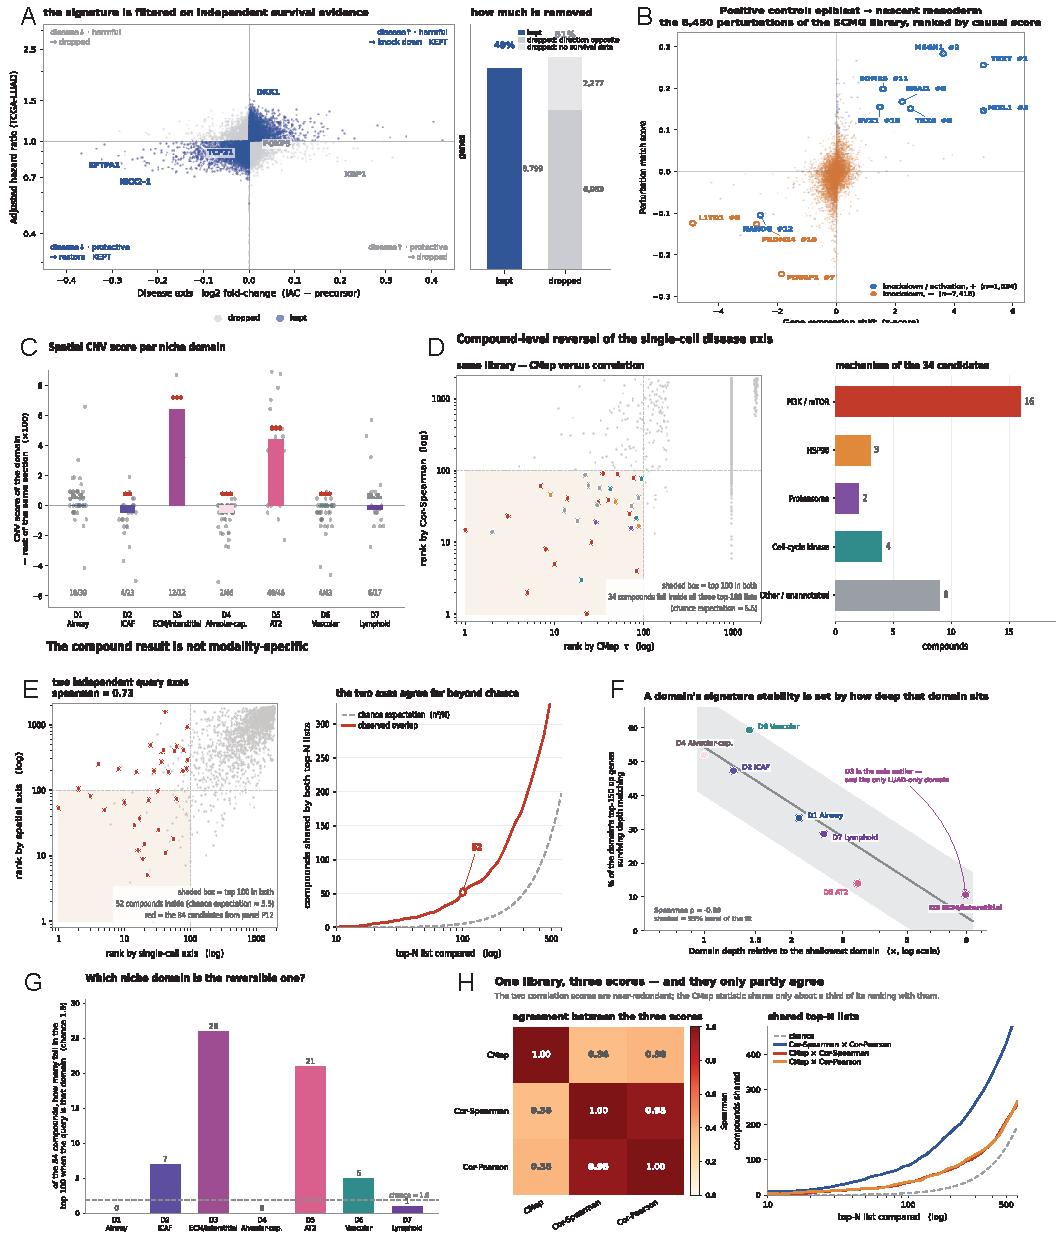
\includegraphics[width=\textwidth]{Fig3}
  \caption{\textbf{\emph{In-silico} reversal of the disease state.}
(\textbf{a}) The query signature is filtered on independent survival evidence: disease
direction against adjusted hazard ratio, with genes whose directions disagree set to zero.
(\textbf{b}) Positive control --- the official epiblast-to-nascent-mesoderm benchmark,
with the known regulators labelled and ranked (TBXT 1st of 8,450).
(\textbf{c}) Spatial copy-number score per domain, each domain compared with the remaining
spots of the same section so that all spots in a comparison share one library.
(\textbf{d}) Compound-level reversal: CMap rank against Cor-Spearman rank for the 1,826
compounds, with the 34 compounds common to all three scoring schemes highlighted, and their
mechanism composition.
(\textbf{e}) The candidate ranking is not modality-specific: a single-cell-derived and a
spatially derived query axis agree at Spearman $\rho=0.735$.
(\textbf{f}) A domain's marker stability scales with its sequencing depth
($\rho=-0.89$; D3 is the sole outlier and the only invasive-restricted domain).
(\textbf{g}) Of the 34 candidates, 26 fall in the top 100 for the ECM/interstitial domain
and 21 for the AT2 domain, against a chance expectation of 1.9.
(\textbf{h}) One library, three scores: the two correlation scores are near-redundant
($\rho=0.950$) whereas the CMap statistic shares only about a third of its ranking with
them.}\label{fig:3}
\end{figure*}


\subsection{Gating of the candidate gene list}

The same disease axis was scored against a gene-perturbation library of 20,345 perturbations
\citep{pan2026scmg} using the authors' causal predictor. The gating framework applied to the
resulting ranking is described here because it converts an ungoverned list into a short one
and because it exposes a failure mode that a naive ranking conceals.

A gene-perturbation score is informative only if the effect depends on the cell type being
perturbed. Every perturbation was therefore scored on a K562 control axis, and those whose
effect was as strong there as on the target axis were removed. Of 9,878 scored entries, 20
were flagged as generalising, 48 were specific to the non-K562 reference, 1,898 were neutral
and 7,912 lacked K562 data and are reported as untested. Applying this gate together with
the survival-direction filter leaves 25 entries supported by all four scoring routes, 111 by
three and 7 by two.

To test whether the candidates act on a compartment rather than on the tissue as a whole,
the disease axis was rebuilt for each of 31 subtypes separately and every perturbation
re-ranked within each axis. Of 1,748 entries reaching the top 100 in at least one cell-type
axis, only two reach it in twenty or more of the 31. One is \emph{SFTPC} knockdown, which
ranks in the top 100 in 22 of 31 axes but fails the direction check, since lowering a
transcript whose high expression is protective does not describe a therapeutic direction.
The other is \emph{STAT1} knockdown (21 of 31 axes; hazard ratio 1.08, consistent with the
required direction). The remaining candidates are largely axis-specific. The headline number
of the ungated ranking is misleading for this reason: ubiquity across cell types is not
evidence of a target, and the entry that appears most broadly reproducible does not survive
the direction filter.

\subsection{Analyses that did not work}

Six further negative results are reported, each with the reason it is believed to have
failed.

\paragraph{Gene-level prediction on the pooled axis.} Applied to the tissue-pooled disease
axis, the pipeline produced a maximum causal score of 0.083 against 1.279 for the official
benchmark on the same implementation, and the distribution on our axis has no high tail,
whereas the benchmark's does. Since the method is demonstrably functional, the pooled axis
has no detectable match to the expression shifts recorded in the library. The
compartment-resolved query does rank, but its survivor count is one. A separate,
self-implemented cosine projection, which omits the causal score's gene-shift term, also
ranked genes, but its significance saturates at the permutation floor (237 of 2,439 genes at
the minimum attainable $p$) and it cannot discriminate.

\paragraph{A developmental trajectory that runs the wrong way.} Using the source study's
approach (monocle3 \citep{cao2019monocle3} with CytoTRACE \citep{gulati2020cytotrace}), the
score is highest rather than lowest in invasive disease: medians are Normal 0.288, AAH
0.374, AIS 0.288, MIA 0.277 and IAC 0.453, a non-monotonic profile with IAC highest. The
reversal is robust, with 22 of 23 patients showing a positive per-patient slope and a
depth-balanced audit finding IAC highest within every depth stratum. The measurement is
nevertheless ambiguous in a way that cannot be resolved. CytoTRACE is constructed from the
number of detected genes, so a high score in invasive disease is equally consistent with
greater transcriptional disorder and with a less differentiated state; two readings fit the
same numbers. Because the analysis measures a stage axis rather than a subtype axis, no
AIC/KAC or tumour labels being available, it can be interpreted neither as evidence against
the source study's trajectory nor as evidence for a different one.

\paragraph{A spectral mechanism that was an artefact of construction.} An initial attempt to
read the trajectory from the spectrum of an optimal-transport operator
\citep{schiebinger2019wot,lange2022cellrank} was abandoned after inspection. Under the stage
partition the coupling matrix is block upper triangular, so transport does not enter the
spectrum; in small independent checks with known row sums the eigenvalue union differed by
$0.000\times10^{0}$ and the number of near-zero eigenvalues equalled the cell count of the
first four stages. The apparent spectral gap was set by a coupling-weight parameter and not
by the data. The result was, on inspection, a property of how the matrix was assembled.

\paragraph{H\&E imaging at this resolution.} A pathology-language model
\citep{huang2023plip} was applied to the H\&E images to ask whether the morphological sequence
could be read directly from the histology. Across twelve independent configurations (six
feature arms crossed with two prompt sets) the best correlation was 0.729, and no setting
exceeded 0.74. The ceiling is set by the model architecture: PLIP takes a 224-pixel input
yielding 49 tokens, so one token spans about 181~$\mu$m of tissue, against the finest
available colour source at 5.670~$\mu$m per pixel. Above that scale the discriminative power
did not vary with detail, and finer sources cannot be tested in this cohort because none
exists.

For the use this study would make of it, the decisive result is that the model did not
resolve the precursor stages. Per-stage means for AAH, AIS and MIA all fell within 0.15 to
0.22 and interleaved with one another, so the three stages that define the sequence are not
separated by this model. What increased with image detail was only the contrast between
invasive disease and everything else, with the benign end depressed, rather than a gradient
across stages.

A search over 1,344 template-and-term combinations identifies what the model is in fact
measuring. The highest raw discrimination, an AUC of 0.972, came from the term
``invasive adenocarcinoma with desmoplastic stroma'', but that term also correlated most
strongly with tissue density ($\rho=0.574$), and projecting the density direction out of its
embedding reduced the AUC to 0.759. A weaker prompt chosen to be density-neutral retained
more of its discrimination under the same projection (raw AUC 0.833, $\rho=0.129$;
projected 0.791). Two independent measurements agree: the lesion score correlates at
$\rho=0.718$ with the tissue fraction of a spot and at $\rho=-0.794$ with an empty-slide
control; and the model does not merely fail to rank precursor lesions above normal lung, it
inverts the comparison, with AAH versus Normal AUCs of 0.28 to 0.32 across prompt sets.
Tumour tissue is itself denser than normal lung, so removing density also removes part of the
true signal and the projected values are a lower bound rather than a target. The relevant
point is that performance here is not separable from how much tissue a spot contains.

To establish that the ceiling reflects resolution rather than the choice of image, every
section was registered from the high-resolution image into the CytAssist frame (56 of 56
passing; Methods) and the same spots were re-scored from four image sources matched by
physical size. The finer source did not improve performance: slice-level correlation was
0.698 for the baseline image, 0.228 for CytAssist, 0.540 for CytAssist contrast-matched to
the baseline, and 0.215 for CytAssist downsampled to the baseline's pixel density. Because
downsampling and raw CytAssist perform alike, the difference is not one of pixel density but
of white balance and contrast between the two products, and matching the contrast recovers
most of it.

The conclusion is correspondingly narrow. At this image scale the model cannot perform the
task this study would require of it, which is to place a lesion on the precursor-to-invasive
axis. That is not a statement that histological detail is uninformative in general: testing
that would require a finer colour source than this cohort provides.

\paragraph{The ligand layer.} NicheNet was used with fibroblasts as receivers, the ten most
abundant non-fibroblast cell types of the ECM/interstitial domain as senders, and the same
data-derived target set. Only five ligands passed the expression and network gates, and none
produced a ligand--target link in the output matrix. Their ligand activities were
correspondingly flat, the best corrected area under the precision--recall curve being 0.093
against a baseline of zero. Since NicheNet's own baseline correction was applied, the
failure lies in the candidate set rather than in the scoring: with five ligands the sender
panel is too thin for the network to resolve anything. Ligand-level inference is the natural
next step, and this is the specific reason it was not pursued here.

\paragraph{A finer spatial resolution that measured sections.} One attempt to ask whether the
RCTD composition space supports more than seven domains pooled spots from all 56 sections
into a single $k$-means and cross-validated the result. It returned a clean optimum, but the
clusters tracked section identity rather than niche. Pooling across sections makes
between-section differences the dominant axis of variation, so the bootstrap measured
whether clusters mixed across sections are stable and not whether the composition space
supports a finer partition. The analysis was superseded by a per-section clustering with the
same $K$ scan, which is the version reported above.

\begin{table*}[!ht]
\centering
\begin{tabularx}{\textwidth}{@{}>{\itshape\raggedright\arraybackslash}p{94pt}>{\raggedright\arraybackslash}p{152pt}X@{}}
\toprule
\tabheadfont Analysis & \tabheadfont What was observed & \tabheadfont Most likely reason, and the check behind it \\
\midrule
Single-cell copy number & no usable malignant/non-malignant separator across six tool families; the one AUROC of 0.5000 was a degeneracy (a single score value for all 19{,}748 cells) & the per-patient benign anchor is unstable: the same 3{,}890 normal cells gave aneuploid calls of 0\%, 13.6\% and 49.8\% in three runs. Not evidence that copy-number differences are absent. \\
\addlinespace[2pt]
Cohort-level spatial copy number & the invasive-vs-precursor difference shrank 71\% after depth matching ($p = 0.092$, CI including zero) & depth and tissue density are the same measurement here. A random subsample reproduced the pre-matching result index by index, so the original effect was depth-driven rather than a sample-size artefact. \\
\addlinespace[2pt]
Copy-number subdomain within AT2 & the score correlates with total UMI at $r = 0.755$, and a count-only split reproduces $\sim$75\% of the AT2 contrast & RNA content and copy-number score are not separable; a high-score subdomain cannot be called a tumour subdomain. \\
\addlinespace[2pt]
Developmental trajectory & the score is highest, not lowest, in invasive disease (0.453 vs 0.288--0.374), robust in 22 of 23 patients & we measure a stage axis, not a subtype axis (no AIC/KAC or tumour labels). The score is built from detected-gene counts, so the same numbers also fit ``more transcriptionally disordered''. \\
\addlinespace[2pt]
Transport-spectrum trajectory & the apparent spectral gap was set by a coupling-weight parameter & under a stage partition the coupling matrix is block upper triangular, so transport never enters the spectrum. A parameter was being read as biology. \\
\addlinespace[2pt]
Gene-level reversal, pooled axis & maximum causal score 0.083 against 1.279 for the official benchmark & the pooled axis has no detectable match in the library. The positive control passes, so this is a statement about the query. \\
\addlinespace[2pt]
Gene-level reversal, per compartment & only two perturbations reach the top 100 in $\geq$20 of 31 subtype axes, and one fails the direction check & ubiquity across compartments is not evidence of a target; the survivor list is a single entry and is reported as an observation. \\
\addlinespace[2pt]
Ligand layer & five ligands passed the expression and network gates; none produced a ligand--target link; best corrected AUPR 0.093 & the sender panel is too thin. The scoring is baseline-corrected, so this is not a scoring artefact. \\
\addlinespace[2pt]
Four spatial programmes by stage & after depth matching the ordering is identical across all ten deciles but does not follow disease progression & depth creates a spurious trend. Reported as a negative control, not as a result. \\
\addlinespace[2pt]
H\&E imaging & best correlation 0.729 across twelve configurations; the three precursor stages fall within 0.15--0.22 and interleave (AAH versus Normal AUC 0.28--0.32); the top-scoring prompt correlates with tissue density at $\rho=0.574$ and falls to 0.759 when that direction is projected out & architectural resolution (181\,$\mu$m per token against 5.670\,$\mu$m per pixel). At this scale the model's performance is not separable from tissue density and it cannot place a lesion on the precursor-to-invasive axis. Does not mean histological detail is uninformative in general. \\
\addlinespace[2pt]
Domain stability gate & cross-seed ARI never reached 0.90 (median 0.782) & the domain definition is method-sensitive (BANKSY 7, RCTD 6, marker-based 5; ARI 0.352). The partition is reported as exploratory. \\
\addlinespace[2pt]
Pooled cross-section clustering & a clean optimum that tracked section identity & pooling sections makes between-section variation the dominant axis; superseded by per-section clustering. \\
\bottomrule
\end{tabularx}
\caption{\textbf{Negative results and the reason we believe each one failed.} The right-hand
column is an assessment, not a measurement: it names the most likely explanation and, where
we could test it, the check that separates an absent signal from a broken method. The
distinction matters because a negative result with a passing positive control constrains the
biology, whereas one without does not.}
\label{tab:negatives}
\end{table*}


\begin{table*}[!ht]
\centering
\begin{tabularx}{\textwidth}{@{}>{\raggedright\arraybackslash}p{116pt}>{\raggedright\arraybackslash}p{104pt}X@{}}
\toprule
\tabheadfont Check & \tabheadfont Compared against & \tabheadfont Result \\
\midrule
\tabgroup{3}{Numerical agreement with the reference implementation}
Weighted-KS statistic & \texttt{signatureSearch} 1.12.0 & max.\ abs.\ difference \num{6.6e-14}; signs agree \num{2000}/\num{2000} \\
Normalised connectivity & \texttt{signatureSearch} 1.12.0 & max.\ abs.\ difference \num{1.2e-13} \\
Causal gene score & authors' Python & Spearman \num{1.00000000}; signs agree 100\% (\num{19819} entries) \\
\addlinespace[3pt]
\tabgroup{3}{Biological positive control}
Official benchmark & epiblast $\rightarrow$ nascent mesoderm & TBXT 1st of \num{8450}; MSGN1 2nd; MIXL1 3rd; POU5F1 7th; SNAI1 9th; EOMES 11th; NANOG 12th; EVX1 15th \\
\addlinespace[3pt]
\tabgroup{3}{Stability and agreement}
Split-half & 4 patient partitions & median $\rho = 0.962$ (one split 0.752); permutation null $\pm0.045$ \\
Cross-modality & single-cell axis vs spatial axis & $\rho = 0.735$; top-100 overlap 52 (chance 5.5) \\
Scoring schemes & CMap vs the two correlations & Cor--Cor $\rho = 0.950$ (433 of top 500 shared); CMap--Cor $\rho = 0.36$--$0.38$ \\
\addlinespace[3pt]
\tabgroup{3}{Geometric self-consistency}
Scale-bar calibration & adjacent-spot spacing $= 100$\,$\mu$m & 1\,px $= 0.2513$\,$\mu$m; full panel 10.9\,mm (11\,mm format) \\
\bottomrule
\end{tabularx}
\caption{\textbf{Method verification and positive controls.} Every numerical check compares
our own implementation with the reference implementation on identical input, so a
discrepancy would be an implementation error rather than a modelling choice. The biological
control establishes that an empty result from this pipeline reflects the query and not the
method.}
\label{tab:validation}
\end{table*}


\section{Discussion}

The central difficulty of this study is that sequencing depth and tissue density are, in
this cohort, the same measurement. A domain's marker stability, the apparent
stage-dependence of the spatial programmes, the cohort-level copy-number difference and the
prognostic weight of one domain's signature all vary with depth, and depth varies with the
amount of tumour in a spot. Adjusting for depth is consequently not a neutral correction: it
removes part of the biological effect together with the technical one. Adjusted estimates
are conservative and may be over-corrected; unadjusted estimates are inflated. Where the
choice is consequential, both are reported rather than one being nominated as correct.

The coupling also accounts for the behaviour of the pathology model, which is the one
result here obtained without any transcriptomic measurement. Its apparent discrimination
was largely a measure of how much tissue a spot contained, and on the axis this study needs,
the separation of precursor from invasive lesions, it failed outright. A model that reads
tissue density will appear to succeed on this disease for as long as density and malignancy
coincide, which is exactly the condition that makes the confound difficult to detect.

This also accounts for the narrower scope of some results relative to the source study.
Where a claim depends on comparing dense with sparse tissue, which in this disease means
comparing invasive with precursor tissue, the design carries the confound in its structure.
The only clean comparisons are those that hold depth fixed, either by pairing within a
section or by matching across sections. That is why the one copy-number result retained is a
within-section comparison, and why the disease-axis queries were constructed by pairing
within patients.

\subsection{What the positive results establish}

Four findings survive the checks applied. First, the tissue resolves into seven recurring
niche domains, six of which are ordinary lung structures and only one of which is confined
to invasive disease. The lymphoid-aggregate domain is present in precursor stages, which
argues against attributing immune aggregation to the onset of malignancy. Second, the
ECM/interstitial programme that distinguishes the invasive domain is itself elevated in
invasive disease within patients (20 of 22), and the result holds when the genes added by
hand are removed and under every leave-one-out variant, so the domain label does not rest on
a hand-picked panel. Third, the spatial copy-number signal lies in the AT2 compartment and
is present before invasion, consistent with AT2 as the cell of origin and with an orthogonal
expression-based classifier. Fourth, a query signature derived from a patient-internal
disease axis and filtered on independent survival evidence returns a reproducible set of 34
compounds, dominated by PI3K/mTOR inhibitors, which act on the ECM/interstitial and AT2
domains rather than on the tissue as a whole.

The candidate list should be read as a hypothesis about a compartment rather than as a
therapy. Several caveats are structural. The compounds act in cancer cell lines and have not
been tested in lung fibroblasts or in any primary tissue. The disease axis against which they
were selected is a tissue-level average, so the candidates reverse the aggregate state and
need not act on any single cell type. The 34 compounds are the intersection of three scoring
schemes, but those schemes share a query and a library and their agreement is therefore a
robustness check rather than three independent measurements. The split-half reproducibility
of 0.962 describes the stability of the ranking under resampling of patients and says
nothing about whether the ranking is biologically correct. No compound reported here has
been tested experimentally.

\subsection{Methodological observations}

Several of the checks applied here are reusable, and the difficulties encountered carry
lessons that are not specific to this dataset.

A positive control with a known answer, run through the identical pipeline, distinguishes
``the method found nothing'' from ``the data contain nothing detectable by this method''.
Without such a control the negative results reported above would be uninterpretable. A
related practice is to inspect the distribution of a summary statistic rather than the
summary alone: an AUROC of exactly 0.5000 in this study was a degeneracy, all cells carrying
one identical value, and not a true null.

Control for a nuisance variable is better served by sensitivity analysis than by a single
adjusted estimate. When a measurement is strongly coupled to such a variable, examining
subsets of the measurement is more informative than adjusting once. In this study, showing
that a result held when the eight hand-added genes of a marker panel were removed, and
across all twenty-two leave-one-out variants, established that the finding did not depend on
the panel's arbitrary members. A related caution applies to sub-clustering: because clusters
are selected on the same data used to test them, per-subtype contrasts carry a
selective-inference penalty that is not corrected here \citep{gao2024selective}, which is
one reason the per-compartment gene list is reported as descriptive.

Two further observations concern how criteria are constructed and reported. A gate that
every configuration passes is not a gate. The spatial-coherence criterion applied here,
which required a partition's coherence to exceed a label-permutation null on at least 90\%
of sections, was passed by essentially every configuration tried, including one that uses no
spatial information at all ($\lambda=0$; coherence 0.54--0.60 against a null 95th percentile
of 0.13--0.18). Tissue expression carries spatial autocorrelation intrinsically, so a purely
expression-based partition clears the null by a wide margin. The criterion can exclude a
grossly anti-spatial partition but cannot demonstrate that spatial information was used;
ranking was accordingly decided by cross-seed stability instead. In addition, a criterion
introduced by the analysts must not be presented as though it carried external authority.
The coherence gate is ours. The source study sets no spatial gate, and the BANKSY authors'
recommendations \citep{singhal2024banksy} concern parameters ($\lambda$, $k_{\text{geom}}$,
resolution) rather than validation criteria.

Finally, a number produced by an optimiser's trajectory is not a measurement. One weighting
parameter carried for a time in this work, $w_{\min}=(1/6)\times0.7^{k}$, is the path the
solver took rather than a quantity estimated from the data, and should not be reported as
though a fit had produced it.

\subsection{Relation to the source study}

This study set out to extend a published description of the disease sequence
\citep{peng2026}. The results agree with it on the identity of the niche structures and on
AT2 as the compartment carrying copy-number signal, and differ in emphasis on three points.
The source study reports a pro-inflammatory niche that is enriched early and less frequent
in invasive disease; our spatial arm does not reproduce that direction. Its developmental
trajectory places the least differentiated state in precursor lesions, whereas ours runs the
other way, although, as noted, the measurement is ambiguous and is not treated as a
refutation. The source study also does not describe ambient-RNA correction, whereas one of
its samples is, in our hands, dominated by ambient signal. These divergences are reported
rather than adjudicated, since each is confounded by a design difference: different
platforms, a stage axis rather than a subtype axis, and different approaches to quality
control.

\subsection{Priorities for further work}

The comparison that would remove the dominant confound is within a single section, comparing
the invasive front with regions of the same section distant from it and holding depth fixed
by construction. That analysis was not performed and is the one we would prioritise next,
together with testing the candidate compounds in primary lung fibroblasts or in organoids
derived from the same patients.

\section{Limitations}

\begin{enumerate}\itemsep2pt

\item \textbf{Depth and density are not separable.} Every analysis in this paper is
affected by the fact that sequencing depth proxies tissue density. Where the choice is
consequential we report both adjusted and unadjusted estimates rather than selecting one.

\item \textbf{No per-cell malignant label.} We do not assign malignant status to any cell,
spot or domain. The copy-number score is reported as a continuous quantity throughout, and
no downstream statistic multiplies it into any other measurement.

\item \textbf{Domain identity is method-sensitive.} BANKSY, RCTD composition and
marker-based clustering resolve 7, 6 and 5 domains respectively, with an adjusted Rand
index of 0.225--0.247 against an RCTD-aligned partition. The seven domains are a working
description, not a unique decomposition.

\item \textbf{The deconvolution reference bounds what deconvolution can report.} The
39-subtype reference has no exhaustion programme, so exhausted T cells are reported under a
naive label. T-cell composition in this paper is a composition in the reference's
vocabulary; functional states not present in the reference are invisible to it, and were
measured separately by signature projection.

\item \textbf{The $K^{*}=7$ partition failed its pre-specified stability gate.} Across
seedings the cross-seed adjusted Rand index never reached 0.90. We report the partition as
exploratory and do not use it as a primary result; the consequences are confined to
descriptions of domain composition. The companion spatial-coherence criterion we also
applied is passed by every configuration tested, including one using no spatial
information, and therefore carries no weight in this cohort.

\item \textbf{One clinical stage is represented by one section.} The Normal arm of the
spatial cohort consists of a single Visium section; MIA is represented by four. Estimates
for these stages should not be quoted on their own. Nuclei are more balanced (92,337
normal nuclei across 23 patients), so the imbalance is specific to the spatial arm.

\item \textbf{Two domain identities were revised during the study.} The D3 domain was
first described as an immune infiltrate, then as a hypoxic/invasive programme, and finally
as ECM/interstitial-enriched after depth matching showed the first two readings to be
driven by depth. Earlier names for this domain should not be used.

\item \textbf{The marker panel for one analysis was hand-curated.} A 22-gene ECM panel
used in the early spatial analyses overlaps the depth-balanced marker set by only 14
genes; the remaining eight were added by us. A sensitivity analysis shows the finding is
unchanged when those eight are removed, or when any single gene is removed, but the panel
itself is not drawn from a single published source.

\item \textbf{Stage comparisons may be contaminated by sample type.} Patient-internal
pairing removes between-patient variation but not the systematic difference between a
precursor lesion and an invasive carcinoma, which is present in every paired comparison.
The consistency of a signal across 22 patients does not protect against this, since every
patient contributes the same kind of contrast.

\item \textbf{The prognostic analysis is exploratory.} Domain marker signatures were used
without a signed pre-registration of the parameterisation, and one domain's result changes
substantially when its signature is replaced by a depth-balanced version. Only the
direction and its robustness are reported for that domain.

\item \textbf{The compound candidates are untested.} They act in cancer cell lines, have
not been assessed in lung fibroblasts or primary tissue, and have no experimental
validation. They are candidate perturbations.

\item \textbf{The gene-level candidate list rests on one entry.} After the specificity gate,
the direction filter and the compartment decomposition, only two perturbations rank in the
top 100 across twenty or more of the 31 subtype axes, and one of the two fails the
direction check. The surviving gene-level claim therefore rests on a single perturbation
(\emph{STAT1} knockdown), which we report as an observation rather than as a target.

\item \textbf{The ligand layer produced nothing.} NicheNet passed only five ligands, none of
which yielded a ligand--target link, so no ligand-level conclusion can be drawn from this
cohort. The failure is traceable to a thin sender panel and is not evidence that no ligand
effect exists.

\item \textbf{The perturbation libraries are not independent.} The gene-level and
compound-level libraries share the query signature, and the three compound scoring schemes
share both the query and the library. Agreement between them is a robustness check, not
independent corroboration. The two libraries are reported side by side and are not used to
validate one another.

\item \textbf{The pooled gene-perturbation query produced no signal.} Its positive control
passes, so the null reflects the query rather than the method, but we cannot distinguish
between ``this cohort's pooled disease axis is not represented in the library'' and ``no
single-gene perturbation of this magnitude exists in the library''. Splitting the query by
compartment recovers a ranking, so the null is specific to the pooled parameterisation
rather than to the library.

\item \textbf{The developmental analysis is ambiguous by construction.} The score we use
is derived from the number of detected genes, so a high value in invasive disease is
equally consistent with greater transcriptional disorder. Two readings fit the same
numbers and we cannot separate them with the available labels.

\item \textbf{The imaging analysis is bounded by resolution, not by biology.} The
H\&E-based classifier ceiling is set by the model architecture against the available image
scale, and the model does not separate the precursor stages from one another at all. The
negative result concerns what this pipeline can extract at this resolution, not what is
present in the tissue; a finer colour source would be needed to test the latter.

\item \textbf{No orthogonal validation.} No result in this paper has been reproduced in an
independent cohort, with a different perturbation library, or experimentally.

\end{enumerate}

\section{Methods}

\subsection{Data}

\paragraph{Primary cohort.} Two modalities from the same patient series were used.
Single-nucleus RNA sequencing (GSE308103) was generated with a fixed RNA-profiling probe
panel rather than a standard 3$'$ or 5$'$ chemistry, so it quantifies a defined set of
18{,}082 genes rather than the whole transcriptome; this is why housekeeping and
mitochondrial transcripts such as \emph{GAPDH}, the ribosomal protein genes and
\emph{MALAT1} are absent by design and are not used in any signature. The series contains
75 samples from 25 patients; 798{,}100 nuclei were called, of which 767{,}839 passed
quality control and 118{,}894 (15.48\%) were called as doublets, leaving
\textbf{413{,}697 nuclei} profiled over 18{,}069 genes for analysis.
Spatial transcriptomics (GSE307534) was generated on the Visium CytAssist platform in the
11\,mm format, 55\,$\mu$m spots on a $128\times112$ grid with a nominal spot-to-spot
distance of 100\,$\mu$m, giving 14{,}336 spots per section across \textbf{56 sections from
25 patients}; the platform implements the spatial-transcriptomics method of
\citet{stahl2016}. The two modalities share \textbf{23 patients}. The clinical sequence is
Normal $\rightarrow$ AAH $\rightarrow$ AIS $\rightarrow$ MIA $\rightarrow$ IAC; the spatial
annotations use the source study's token \texttt{LUAD} for the invasive stage, which we map
to IAC throughout. Section counts per stage are Normal 1, AAH 11, AIS 14, MIA 4, IAC 26
(Table~\ref{tab:cohort}).

\paragraph{External statistics.} Prognostic filtering used TCGA-LUAD
\citep{tcga2014luad} in its archived form: expression and clinical matrices only, giving
\textbf{483 patients and 177 deaths} (36.6\%; 381 patients and 143 events for disease-free
survival). The mutation archive in that distribution is a zero-byte file, so no
mutation-derived quantity (TMB, driver status) enters any analysis.

\paragraph{Perturbation resources.} Two libraries were queried. The compound library is
LINCS L1000 Level 5 (GSE70138; 118{,}050 signatures $\times$ 12{,}328 genes, 1{,}826
unique perturbagens across 41 cell lines) \citep{subramanian2017}; we rebuilt it locally
as described below rather than querying the CLUE service. The gene-level library is SCMG
\citep{pan2026scmg} (20{,}345 perturbations $\times$ 18{,}108 genes), used with the
authors' \texttt{CausalGenePredictor} and their reference cell-state manifold.

\paragraph{Annotation references.} Cell-type annotation was cross-checked against the
CellTypist \texttt{Human\_Lung\_Atlas} model \citep{dominguezconde2022celltypist}, itself
built on the HLCA \citep{sikkema2023}. Ligand analysis used the NicheNet human
ligand--receptor network and ligand--target matrix \citep{browaeys2020nichenet}.

\paragraph{Resources evaluated and not used.} Three external resources were assessed and
rejected, and we record them so that their absence is not read as an oversight. An external
normal-lung Visium series (GSE248082) was examined as a benign anchor for the copy-number
arm; its two usable sections failed a two-way health check (the held-out section scored
above threshold in both directions), so no external anchor is claimed. An external
lymph-node-metastasis series initially earmarked for the spatial cohort proved, on
inspection, to be breast rather than lung cancer and was removed. Three public single-cell
cohorts considered in the study's first design were moved out of scope when the paired
series became available, and were never analysed. No GWAS, eQTL, docking or structural data
entered this work.

\begin{table*}[!ht]
\centering
\begin{tabular*}{\textwidth}{@{\extracolsep{\fill}}l >{\raggedright\arraybackslash}p{172pt} >{\raggedright\arraybackslash}p{172pt}@{}}
\toprule
\tabheadfont Item & \tabheadfont Single-nucleus RNA-seq & \tabheadfont Spatial transcriptomics \\
\midrule
Accession & GSE308103 & GSE307534 \\
Platform & fixed RNA profiling & Visium CytAssist, 11\,mm \\
Feature space & 18{,}069 genes analysed & 18{,}085 probes \\
Samples & 75 & 56 sections \\
Patients & 25 & 25 \\
\addlinespace[3pt]
Units called & 798{,}100 nuclei & 14{,}336 spots per section \\
Retained after QC & 767{,}839 (96.2\%) & 95.03\% of spots \\
Doublet rate & 15.48\% & --- \\
Analysed & \textbf{413{,}697 nuclei} & all 56 sections \\
Grid and spacing & --- & $128\times112$; 100\,$\mu$m \\
\addlinespace[3pt]
Patients in both modalities & \multicolumn{2}{l}{23} \\
\bottomrule
\multicolumn{3}{@{}l}{\footnotesize\itshape Sections per stage: Normal 1 \quad AAH 11 \quad AIS 14 \quad MIA 4 \quad IAC 26 (source token \texttt{LUAD})} \\
\end{tabular*}
\caption{\textbf{Cohort and data sources.} Both modalities are public, come from the same
patient series, and share 23 patients. Both are probe-based assays rather than
whole-transcriptome chemistries, so each has a defined feature space. The invasive stage is
labelled \texttt{LUAD} in the source annotations and is mapped to IAC throughout. Normal is
represented by a single spatial section and MIA by four, so estimates for these two stages
should not be quoted on their own.}
\label{tab:cohort}
\end{table*}


% 参数表：与队列表相邻放在 Methods 前段，避免落到文末产生整页空白；
% 编号仍按正文首次引用顺序为 Table 6。
\begin{table*}[!ht]
\centering
\begin{tabularx}{\textwidth}{@{}>{\raggedright\arraybackslash}p{68pt}>{\raggedright\arraybackslash}p{78pt}>{\raggedright\arraybackslash}p{104pt}>{\centering\arraybackslash}p{20pt}X@{}}
\toprule
\tabheadfont Arm & \tabheadfont Parameter & \tabheadfont Value & \tabheadfont Src. & \tabheadfont Note \\
\midrule
\tabgroup{5}{Single-cell processing}
QC & retained nuclei & 399{,}579 & S & 15.48\% doublet rate; per-sample MAD \\
Clustering & L2 subtypes & 39 & S & endothelial and myeloid panels rebuilt \\
Integration & batch variable & sample ID & P & Harmony, rest at defaults \\
\addlinespace[3pt]
\tabgroup{5}{Spatial domains (BANKSY)}
Domain search & $\lambda$ & 0.2 & P & authors' recommendation for 55\,$\mu$m Visium \\
 & $k_{\text{geom}}$ & 18 & P & authors' recommendation \\
 & resolution & 0.5 & P & within the source study's range \\
Consensus & seeds & 5 & S & cross-seed agreement, per section \\
Archetypes & $K^{*}$ & 7 & S & stability 0.945 (0.814 at $K=8$) \\
\addlinespace[3pt]
\tabgroup{5}{Spatial deconvolution}
Reference & subtypes & 39 & S & a 6-lineage reference is also run \\
Epithelial call & rule & $\arg\max =$ epithelial & S & fixed before the cohort run \\
Spot mask & threshold & 500 counts / 200 genes / MT 0.15 & S & removes 4.97\% of spots \\
\addlinespace[3pt]
\tabgroup{5}{Copy-number inference}
Engine & tool & fastCNV & P & DOI 10.1186/s13073-026-01731-w \\
Chromosomes & filter & drop chrY, chrM & P & engine behaviour \\
Domain contrast & design & within-section pairing & S & removes depth by construction \\
\addlinespace[3pt]
\tabgroup{5}{Query signature}
Construction & axis & invasive $-$ precursor, median over patients & S & 16{,}104 genes \\
Survival filter & rule & disease-up needs HR$>$1; disease-down needs HR$<$1 & S & removes 51\% of genes \\
\addlinespace[3pt]
\tabgroup{5}{Perturbation querying}
Compound library & LINCS L1000 L5 & 118{,}050 $\times$ 12{,}328; 1{,}826 compounds & P & GSE70138 \\
 & scoring & CMap $\tau$; Spearman; Pearson & P & \texttt{signatureSearch} 1.12.0 \\
Gene library & SCMG & 20{,}345 perturbations & P & MIT-licensed \\
Gating & specificity & K562 control axis & S & removes 20 generalising entries \\
 & compartment & per-subtype axes (31) & S & top-100 counted per axis \\
Null models & permutations & 1{,}000 signature layer & T & \texttt{signatureSearch} default \\
Reproducibility & split-half & 4 partitions & S & reported individually \\
\bottomrule
\end{tabularx}
\caption{\textbf{Analysis parameters and their provenance.} Each parameter is labelled by
its source: \textbf{P}~= stated in a source paper or software publication, \textbf{T}~=
software default rather than a published recommendation, \textbf{S}~= fixed by us and
recorded in the analysis log. The distinction is drawn because most of the consequential
settings in this study are ours rather than the field's.}
\label{tab:params}
\end{table*}


\subsection{Single-cell processing}

After quality control and doublet removal 413,697 nuclei were retained. Contaminant and
low-quality clusters were then excluded, leaving 399,579 nuclei in the six mutually
exclusive lineage subsets that the atlas is built on. Expression was
normalised to counts per 10,000 with a $\log(1+x)$ transform (CP10K+log1p) throughout. The
atlas was built with Seurat \citep{hao2024seurat} using the regularised negative-binomial
variance-stabilising transform \citep{hafemeister2019sctransform} with \texttt{glmGamPoi}
\citep{ahlmanneltze2021glmgampoi} for parameter fitting, and integrated across samples with
Harmony \citep{korsunsky2019harmony}. Doublets were called with scDblFinder
\citep{germain2021scdblfinder}. An independent second caller was attempted but could not
serve as a cross-check: Scrublet \citep{wolock2019scrublet} reached a maximum score of
0.495 against its automatic threshold of 0.556 on these nuclei and therefore called zero
doublets in all 75 samples, a consequence of how sparse these profiles are rather than
evidence against the scDblFinder calls. The atlas was clustered per lineage, yielding 39
second-level
(L2) subtypes. Endothelial and myeloid marker panels were rebuilt before downstream
analysis: the published table provided six canonical genes per endothelial subtype, which
we expanded to as many as twenty genes per subtype across nine endothelial types; the
myeloid panel was expanded analogously, drawing on the human lung atlases
\citep{travaglini2020,habermann2020,vieirabraga2019,sikkema2023} and, for the epithelial
subtypes, on the lung adenocarcinoma atlas \citep{han2024,sinjab2021}. Automated annotation
against the HLCA reference used CellTypist \citep{dominguezconde2022celltypist}. All
reported subtype compositions use the expanded panels.

Ambient RNA was assessed in one precursor sample (P24) by three independent checks
(patient-level rank of the suspect programme, comparison against a matched negative-control
gene set, and an independent readout from a separate region of the same block). The sample
was retained with an annotation and all B/plasma-dependent conclusions are reported with
and without it.

\subsection{Spatial domain identification}

Spatial domains were identified with BANKSY \citep{singhal2024banksy} on each section
independently. The main
configuration was fixed at $\lambda=0.2$, $k_{\text{geom}}=18$ and resolution 0.5, chosen
because the authors recommend $\lambda\approx0.2$ for domain segmentation on 55\,$\mu$m
Visium and because higher $\lambda$ values, which the source study used, down-weight the
cell's own expression towards zero. Cross-seed consensus over five seeds produced 434
domain-level clusters across 56 sections; these were collapsed to archetypes by
profile-based clustering, giving $K^{*}=7$ at a subsampling stability of 0.945 (re-clustering on a random 80\% of
domains, 100 iterations); the cross-seed adjusted Rand index of the per-section domain
calls is a separate quantity and is lower (median 0.782). Stability
falls below 0.814 at $K=8$. A descriptive optimum exists at $K=6$ (0.966) but was not
adopted, since the selection rule took the largest $K$ passing the stability threshold.
Consensus stability was scored with the proportion-of-ambiguous-clustering statistic
\citep{senbabaoglu2014pac}.

A spatial-coherence criterion was also computed: per section, the mean coherence of the
partition was required to exceed the 95th percentile of a label-permutation null, with at
least 90\% of sections passing. This criterion is our own construction, not one recommended
by the source study or by the BANKSY authors, and it is not used to select the
configuration (see Discussion).

\subsection{Spatial deconvolution}

Spot composition was estimated with RCTD \citep{cable2022rctd} against a 39-subtype
reference, using the
full-section non-epithelial compartment as the reference for the copy-number arm (the
arm using each patient's own benign anchor covers only 10 of 25 cases). Spots were called
epithelial when the epithelial subtype had the highest weight; this criterion was fixed
before the cohort run. A spot mask was applied at thresholds of 500 counts, 200 genes and
0.15 mitochondrial fraction, removing 4.97\% of spots cohort-wide. This is higher than the
1.05\% reported by the source study; the difference is attributable to uneven per-section
depth rather than to the rule, and is recorded as a known discrepancy.

Two consequences of the mask are guarded explicitly. Per-section removal rates range from
0.02\% to 29.6\%, so a section in which a domain occupies little area may simply have had
more of itself masked; coverage is therefore reported per section and a small domain area is
never read as evidence that the niche is rare. And because the 56 sections come from 25
patients, every cross-section summary is clustered by patient, since two or three sections from
one patient are not independent samples.

\subsection{Depth matching}

Two independent estimators were used. In the first, spots were binned into per-slide deciles
of nUMI and compared only within bins. In the second, each gene was regressed on
$\log_{10}(\text{nUMI})$ per slide with a cubic term, and the domain-versus-rest ranking was
recomputed on the residuals. A gene was counted as surviving if it remained in the domain's
top 150 up-genes. The two estimators agree almost gene-for-gene.

\subsection{Spatial copy-number inference}

Copy-number scores were computed with fastCNV \citep{cabrejas2026fastcnv}. The engine
discards chrY and chrM, and its classification
output is a direction call rather than a malignancy determination; we use only the
continuous per-spot score. Domain-level comparisons pair each spot's score against the
median of the remaining spots in the same section, which removes depth by construction.
Significance was assessed per domain by a two-sided sign test over sections, with
Benjamini--Hochberg control where families of tests are reported
\citep{benjamini1995fdr}. Spatial neighbourhood statistics used Squidpy
\citep{palla2022squidpy}. Three further copy-number tools were evaluated and excluded
because each requires aligned reads rather than an expression matrix (Numbat
\citep{gao2023numbat}, HoneyBADGER \citep{fan2018honeybadger} and CaSpER
\citep{serinharmanci2020caspER}), as was SCEVAN \citep{defalco2023scevan}, which was
pre-registered but not run.

\subsection{Prognostic analysis}

Survival analysis used TCGA-LUAD \citep{tcga2014luad} (483 patients, 177 deaths;
disease-free survival: 381 patients, 143 events, censored at last follow-up), with Cox
proportional-hazards models fitted in R's \texttt{survival} package
\citep{therneau2000survival}. For each domain, the top-30 marker genes
were standardised across samples and averaged into a signature score. Univariate Cox models
were fitted both continuously (hazard ratio per standard deviation) and on a median split
(reference group: low). Hazard ratios for the adjusted models controlled for stage, age and
sex.

\subsection{Query signature construction}

For each patient, the disease axis was computed as the mean expression of invasive cells
minus that of precursor cells, and the median across patients was taken, giving an
18,069-gene vector, of which 16,104 are represented in the SCMG library. This axis was
filtered on independent survival evidence: a gene rising
in disease was retained only if its adjusted hazard ratio exceeded 1, and a gene falling in
disease only if it fell below 1; all others were set to zero. Of 18,069 genes, 8,799 were
retained (51\% removed overall; 44\% of the 15,792 genes with survival annotation).
A second, spatial query axis was constructed by comparing invasive and precursor spots
within nUMI deciles per section, merging deciles weighted by the smaller group size, and
removing immunoglobulin, mitochondrial and antibody-probe rows.

\subsection{A local compound-perturbation database}

The standard way to query a disease signature against LINCS is the CLUE service
(clue.io). Its scoring service was retired on 2026-01-31: the site still serves data
downloads, but it no longer accepts scoring jobs, and submission requests are refused
(HTTP 401). Rather than depend on a service that can no longer do the work, we rebuilt the
query resource locally, which has the further advantage that the exact library state is
fixed, versioned and re-runnable rather than whatever the remote service happens to serve
on a given day.

The database is a \texttt{signatureSearch}-format HDF5 file built directly from the LINCS
L1000 Level 5 Z-score matrix (GSE70138, release 2017-03-06). It stores the assay as a
genes $\times$ signatures array of 12{,}328 Entrez genes by 118{,}050 signatures, with
columns keyed by perturbagen, cell line and perturbation type; file size is 5.9\,GB.
Building it through R (\texttt{build\_custom\_db}) was abandoned because the required
compression and index handling failed and the per-column writer was prohibitively slow; the
file used here is written directly with \texttt{h5py}, which takes 26\,s. The database
itself is excluded from the repository, being 5.9\,GB and regenerable from the two tracked
build scripts. The \texttt{padj} slot is deliberately omitted because the scoring functions
used here do not read it.

Two access paths exist over the same underlying LINCS data, and it matters which analysis
used which. The disease-axis query, the spatial-axis query and the split-half stability
check were run through this local database using the official \texttt{signatureSearch}
package. The domain-signature query and all depth-matched sensitivity runs were run
directly on the source matrix through our own implementation of the CMap statistic. Both
paths are cross-validated against the official implementation (Table~\ref{tab:validation}).

\subsection{Slide registration}

The CytAssist images are the finer of the two available H\&E sources, but Space Ranger ships
no transform between them and the spot coordinate frame, so the mapping had to be measured.
We built a registration pipeline that places the high-resolution \texttt{hires} image into
the CytAssist pixel frame under a similarity transform with an optional horizontal
reflection,
$\text{cytassist} = s \cdot R(\theta) \cdot M \cdot \text{hires} + t$.

Three features make the search tractable rather than a blind optimisation. First, the scale
is not searched: it is computed analytically for each section from the shipped
scalefactors, $s_{\text{pred}} = (\text{fullres}\,\mu\text{m/px} \div \text{hires
scalefactor}) \div \text{CytAssist}\,\mu\text{m/px}$, with the CytAssist constant
4.6233\,$\mu$m/px; the search then only refines $\pm3\%$ around this value, and in the
final solution all 56 sections land within 1\% of it. Second, the rotation resolves to
essentially a binary choice: every section's fitted $\theta$ lies within 5$^\circ$ of
0$^\circ$ or 180$^\circ$, and the reflection is applied to 53 of 56 sections. Third, the
search is a coarse-to-fine pyramid over translation, obtained by phase correlation, scored
by a masked normalised cross-correlation of high-pass-filtered greyscale content (search
$\sigma = 12$, verification $\sigma = 4$).

Registration quality was established by three independent checks rather than one. The
adopted transform must score a fine-scale high-pass correlation of at least 0.10 and at
least three times the score of the competing reflection branch; this gate separates, by a
wide margin, the sections that the initial run failed on (the 52 passing sections have
correlation $\geq 0.19$ and separation $\geq 7.0$, while the four failures had separation
$\leq 1.4$ and were re-solved with a tissue-outline overlap metric). Second, the same
physical spot was cropped from both sources and compared directly, with the coordinate grid
propagated through the full transform; the fitted affine reproduces the grid to within
0.18\,px everywhere. Third, the residual was measured on the final solution as a translation field: the
residual translation is within one pixel on 46 of 56 sections, and three pixels or less on
the remainder, and where the field could be fitted it shows no residual rotation
($|\phi| < 0.1^\circ$) and no residual scale ($k$ within $\pm0.13\%$). At the CytAssist
scale of 4.6233\,$\mu$m per pixel this places even the largest residual well inside a spot
radius, so no spot is assigned to a neighbouring spot's tissue. All 56 sections pass. The
pipeline was used to align the same spots across image sources for the H\&E audit reported
in Results; it is retained in the repository.

\subsection{Perturbation scoring}

Compound scoring used the LINCS L1000 Level 5 library \citep{subramanian2017} (118,050
signatures $\times$ 12,328 genes; 1,826 compounds) through \texttt{signatureSearch}
\citep{duan2020signaturesearch} 1.12.0 with three schemes: the CMap weighted-KS statistic
($\tau$; the statistic originates in GSEA \citep{subramanian2005gsea}) on top-150 up/down
gene sets, and Spearman and Pearson correlation on the full numeric vector. Scores were
aggregated per compound by the median across cell lines. Gene-level scoring used the SCMG
library (20,345 gene perturbations)
with the authors' \texttt{CausalGenePredictor}
($\cos \times \text{perturbation sign} \times \text{gene-shift } z$), the authors' reference
manifold and their gene standard deviations.

\subsection{Positive control and numerical verification}

The pipeline was verified in two ways before interpretation. Numerically, our weighted-KS
implementation was compared against \texttt{signatureSearch} 1.12.0
(maximum absolute difference $6.6\times10^{-14}$; signs agreeing for 2000/2000
comparisons; the fast implementation used for the cross-check was \texttt{fgsea}
\citep{korotkevich2016fgsea}), and our vectorised causal score against the authors' Python
implementation
(Spearman 1.00000000 over 19,819 entries). Biologically, the official
epiblast-to-nascent-mesoderm benchmark was reproduced with the authors' own manifold and
standard deviations; the known regulators rank 1st (TBXT, of 8,450), 2nd (MSGN1), 3rd
(MIXL1), 7th (POU5F1), 9th (SNAI1), 11th (EOMES), 12th (NANOG) and 15th (EVX1).

\subsection{Candidate gating and compartment decomposition}

Gene-level candidates passed three additional gates. First, a specificity gate: each
perturbation was scored on a K562 control axis, and an entry whose effect there was as
strong as on the target axis was flagged as generalising and excluded; entries without
K562 data are reported as untested. Second, a compartment decomposition: the disease axis
was rebuilt independently for each of 31 subtypes (mean expression difference between
invasive and precursor cells within the subtype, median across patients) and every
perturbation was re-ranked within each axis; an entry was counted as top-100 for a subtype
at that rank. Third, a survival-direction check: a knockdown was kept only for genes whose
increased expression predicts worse outcome, and an overexpression only for the converse.

\subsection{Ligand analysis}

Ligand-level analysis used NicheNet \citep{browaeys2020nichenet} with the default human
ligand--receptor network and
ligand--target matrix. Fibroblasts were the receiver; the sender panel was the ten most
abundant non-fibroblast subtypes of the ECM/interstitial domain. The target set was the
top-200 up-genes of the data-derived disease axis, not a hand-written list. Candidate
ligands were required to be expressed above $\log(1+\text{CP10K})>0.1$ in at least one
sender and to be present in the ligand--receptor network.

\subsection{Reproducibility checks}

Split-half reproducibility used four random partitions of patients; each half was scored
against LINCS independently, and the Spearman correlation between the two rankings was
compared against a null formed by permuting one half's ranking (300 permutations).
Cross-modality agreement compared the single-cell-axis and spatial-axis compound rankings
by Spearman correlation and by top-$N$ overlap against a chance expectation of $N^2/118{,}050$.
Scale bars in spatial figures were calibrated per section from the median centre-to-centre
distance of adjacent in-tissue spots, which is nominally 100\,$\mu$m; this yields
1\,pixel $=0.2513\,\mu$m and a full-panel width of 10.9\,mm, consistent with the 11\,mm
capture format.

\subsection{Software}

Analyses used R 4.2.2 (Seurat, spacexr, BANKSY, Squidpy's R counterparts,
\texttt{signatureSearch} 1.12.0, survival), Python 3.8 (numpy, scipy, scanpy, h5py) and the
SCMG implementation \citep{pan2026scmg,xingjiepan_scmg}.
All figure code is in the accompanying repository. Table~\ref{tab:params} lists every
consequential parameter together with its provenance.




% 把前面所有尚未落位的浮动体（表 6 等）强制在这里排空，
% 否则它们会漂到文献区里，看起来像"表在引用里面"。
\FloatBarrier

\section*{Data and code availability}
Raw data are public: single-nucleus RNA sequencing (GSE308103) and Visium spatial
transcriptomics (GSE307534). All analysis code, including the scripts that generate every
figure, together with the provenance records for each analysis parameter, is available at
\url{https://github.com/etonsalmon160-source/luad-invasion-v2}. Large intermediate objects
are excluded from the repository because they are regenerable from that code; the exclusion
list records, for each omitted object, the script that rebuilds it.
Supplementary Table~S1 lists the 39 subtypes of the deconvolution reference. The other
derived tables referred to in the text --- per-section copy-number deltas, domain
composition summaries and survival model outputs --- are provided in the repository
alongside the scripts that generate them.

\section*{Funding}
This work received no specific grant from any funding agency in the public, commercial or
not-for-profit sectors.

\section*{Acknowledgements}
The authors thank the colleagues who supported this work despite the absence of dedicated
funding. We are grateful to the senior academic who writes on Bilibili as ``Unshakeable
Saury'', whose understanding and encouragement sustained the project, and to fellow
researchers at Shanghai Jiao Tong University and at Huazhong University of Science and
Technology, whose ideas and technical assistance shaped it. We thank the wider academic
community for recognising this work and for maintaining the decentralised environment in
which it was carried out.

\section*{Author contributions}
\textbf{Z. Li:} conceived and designed the study, performed the computational analyses,
interpreted the results and wrote the manuscript. \textbf{J. Yang:} built and maintained
the computing environment, including server resource provisioning, software setup and
network configuration, and provided the computational infrastructure on which the analyses
were run.

\section*{Use of AI tools}
Claude Code (Anthropic) and DeepSeek were used to write the analysis code and to polish
the language of the manuscript. The study was conceived and designed by the authors; the
analytical strategy, the analysis gates and all thresholds were specified by the authors
and were not determined by the AI tools. All results passed multi-stage review by the
authors before being reported, and the authors take full responsibility for the content of
the manuscript.

\section*{Ethics statement}
This work is a secondary analysis of de-identified, publicly available human data
(GSE308103 and GSE307534). No new human specimens were collected, and no new ethical
approval was required. No animals were used.

\section*{Competing interests}
The authors declare no competing interests.


\bibliography{refs}

\end{document}
